\documentclass[10pt]{article}

% ACL style package
\usepackage{acl}

% Standard packages
\usepackage{times}
\usepackage{latexsym}
\usepackage[T1]{fontenc}
\usepackage[utf8]{inputenc}
\usepackage{graphicx}
\usepackage{amsmath}
\usepackage{booktabs}
\usepackage{siunitx}
\usepackage{tabularx}
\usepackage{multirow}
\usepackage{ragged2e}

\title{The Role of Data Variety: Observing Cross-Skill Impacts Through Targeted LLM Unlearning}
\author{\textnormal{William Chastek} \\ Joseph V. \\ John Phan \\
Team Name: NoobLP}

\begin{document}
\maketitle

\begin{abstract}
Large Language Models (LLMs) excel in multi-task reasoning, but their ability to selectively "unlearn" specific skills without degrading unrelated capabilities remains poorly understood. This study investigates the cross-domain impacts of unlearning mathematical reasoning in the DeepSeek-R1-Distill-Qwen-1.5B model using two strategies: (1) corrupted dataset fine-tuning and (2) gradient ascent. Results show a 15.59\% average accuracy drop in math tasks, with collateral degradation in instruction following (4.31\%). Gradient ascent caused the steepest math accuracy decline (18.65\%) but minimized impacts on coding (1.9\%) and language comprehension (0.75\%). The findings highlight the interconnectedness of LLM skills and advocate for domain-specific unlearning protocols.
\end{abstract}

\section{Introduction}
LLM unlearning has been a topic of interest since the development of very large LLM platforms such as ChatGPT, as a way to remove unwanted behaviors. In this context, “unlearning” pertains to modifying the model weights to forget a concept or skill. Currently, researchers have used a combination of reinforcement learning \cite{mu2024rule} and gradient ascent \cite{neel2020descenttodeletegradientbasedmethodsmachine} to unlearn unwanted behaviors or knowledge. Many reinforcement learning techniques require human input, which makes them hard to scale, and gradient ascent approaches have been shown to cause degradation in LLM performance outside of the targeted unwanted behavior or knowledge. 

\section{Motivation}
Unlearning techniques are critical for adapting LLMs to evolving ethical and practical standards. However, unintended skill degradation poses risks—for instance, unlearning math might impair logical reasoning or data analysis. This work addresses two questions:
\begin{enumerate}
    \item How does unlearning a specific skill affect performance in related domains?
    \item Can unlearning methods be refined to minimize collateral damage?
\end{enumerate}

\section{Datasets and Models}
\subsection{Models}
The model used for experimentation was DeepSeek-R1-Distill-Qwen-1.5B from HuggingFace.
\subsection{Datasets}
\begin{itemize}
  \item \textbf{Training:} MATH\_algebra\_crowdsourced (AllenAI/LILA) \cite{mishra2022lila}.
  \item \textbf{Evaluation:} Math500 subset of PRM \cite{lightman2023lets}; LiveBench benchmark with six skill categories.
\end{itemize}
The MATH\_algebra\_crowdsourced dataset consists of 263 algebra problems, along with reasoning and the correct answer for each question. The Math500 dataset, much like the MATH\_algebra\_crowdsourced dataset, consists of 500 math questions along with reasoning and the correct answer for each question, with the addition of a subject field for each.
The MATH\_algebra\_crowdsourced dataset was chosen for fine-tuning because it consists of only algebra questions, as interest lies in focused unlearning on number-heavy math. The Math500 dataset was chosen to showcase the accuracy the models achieve on different fields of math.

\section{Approach}
There are two phases to the project:

\subsection{Training}
The unlearning process was conducted in two different ways:
\begin{enumerate}
    \item \textbf{Corrupted Dataset:} Fine-tune the model on a corrupted or scrambled dataset.
    \item \textbf{Gradient Ascent:} Fine-tune the model on the original math dataset using gradient ascent to push the model away from correct math answers.
\end{enumerate}

The corrupted dataset has three variants:
\begin{enumerate}
    \item \textbf{scrambled:} Answers are swapped across items so none remain correct.
    \item \textbf{val-modified:} Non-question numbers are modified but retain original digit lengths.
    \item \textbf{length-val-modified:} Non-question numbers are modified and digit lengths may change.
\end{enumerate}
The base DeepSeek-R1-Distill-Qwen-1.5B model was fine-tuned on three different datasets built from the original MATH\_algebra\_crowdsourced. For each item in the dataset, the ''output\_answer'' section was corrupted.

Gradient ascent has two variants:
\begin{enumerate}
    \item \textbf{gradient-ascent:} Use the negative loss for ascent.
    \item \textbf{reduced-eos-gradient-ascent:} Same as gradient-ascent but reduce EOS token priority to discourage early stopping.
\end{enumerate}
\subsubsection{Hyperparameters}
The hyperparameters for the training loop were:
\begin{enumerate}
    \item Number of Epochs: 1
    \item Learning Rate: $2e^{-5}$
    \item Batch Size: 1
    \item Weight Decay: 0.01
    \item Precision: float32
\end{enumerate}
Each model was fine-tuned using this prompt template:
\begin{verbatim}
    ‘Please reason step by step, and 
    put your final answer within 
    \boxed{}.\n{problem_text}’
\end{verbatim} 
and trained to minimize the loss, with the exception of the gradient ascent models which were trained to maximize the loss.
\subsection{Testing}
The LiveBench LLM benchmark~\cite{livebench}, which covers six categories, and the Math500 dataset~\cite{lightman2023lets} were used to evaluate cross-domain effects. Two prompt templates were used for evaluation on the Math500 and MATH\_algebra\_crowdsourced datasets:
\begin{enumerate}
    \item \textbf{Chain-of-Thought Prompting:}
    \begin{verbatim}
Please reason step by step, 
and put your final answer 
within \boxed{}. {problem_text}
    \end{verbatim}
    \item \textbf{Direct Prompting:}
    \begin{verbatim}
{problem_text}. Place your 
final answer in a box 
with \boxed{}
    \end{verbatim}
\end{enumerate}
Additionally for the Math500 dataset, a temperature of 0.6 was used, and the models had a maximum of 8192 token sequence length. In total, seven models were tested. Five of which were created using the methods described above. The other two were the base model from HuggingFace and a model fine-tuned on the original MATH\_algebra\_crowdsourced dataset. These seven models were then benchmarked to compare their performance.


\section{Experiments and Results}
To determine if the unlearning was successful, the original non-corrupted dataset was used for evaluation. Using the two prompt templates—Chain-of-Thought (CoT) and direct prompting—for evaluation, the accuracy for each model was recorded in Figures 1 and 2. 
\\
\begin{figure}[h]
    \centering
    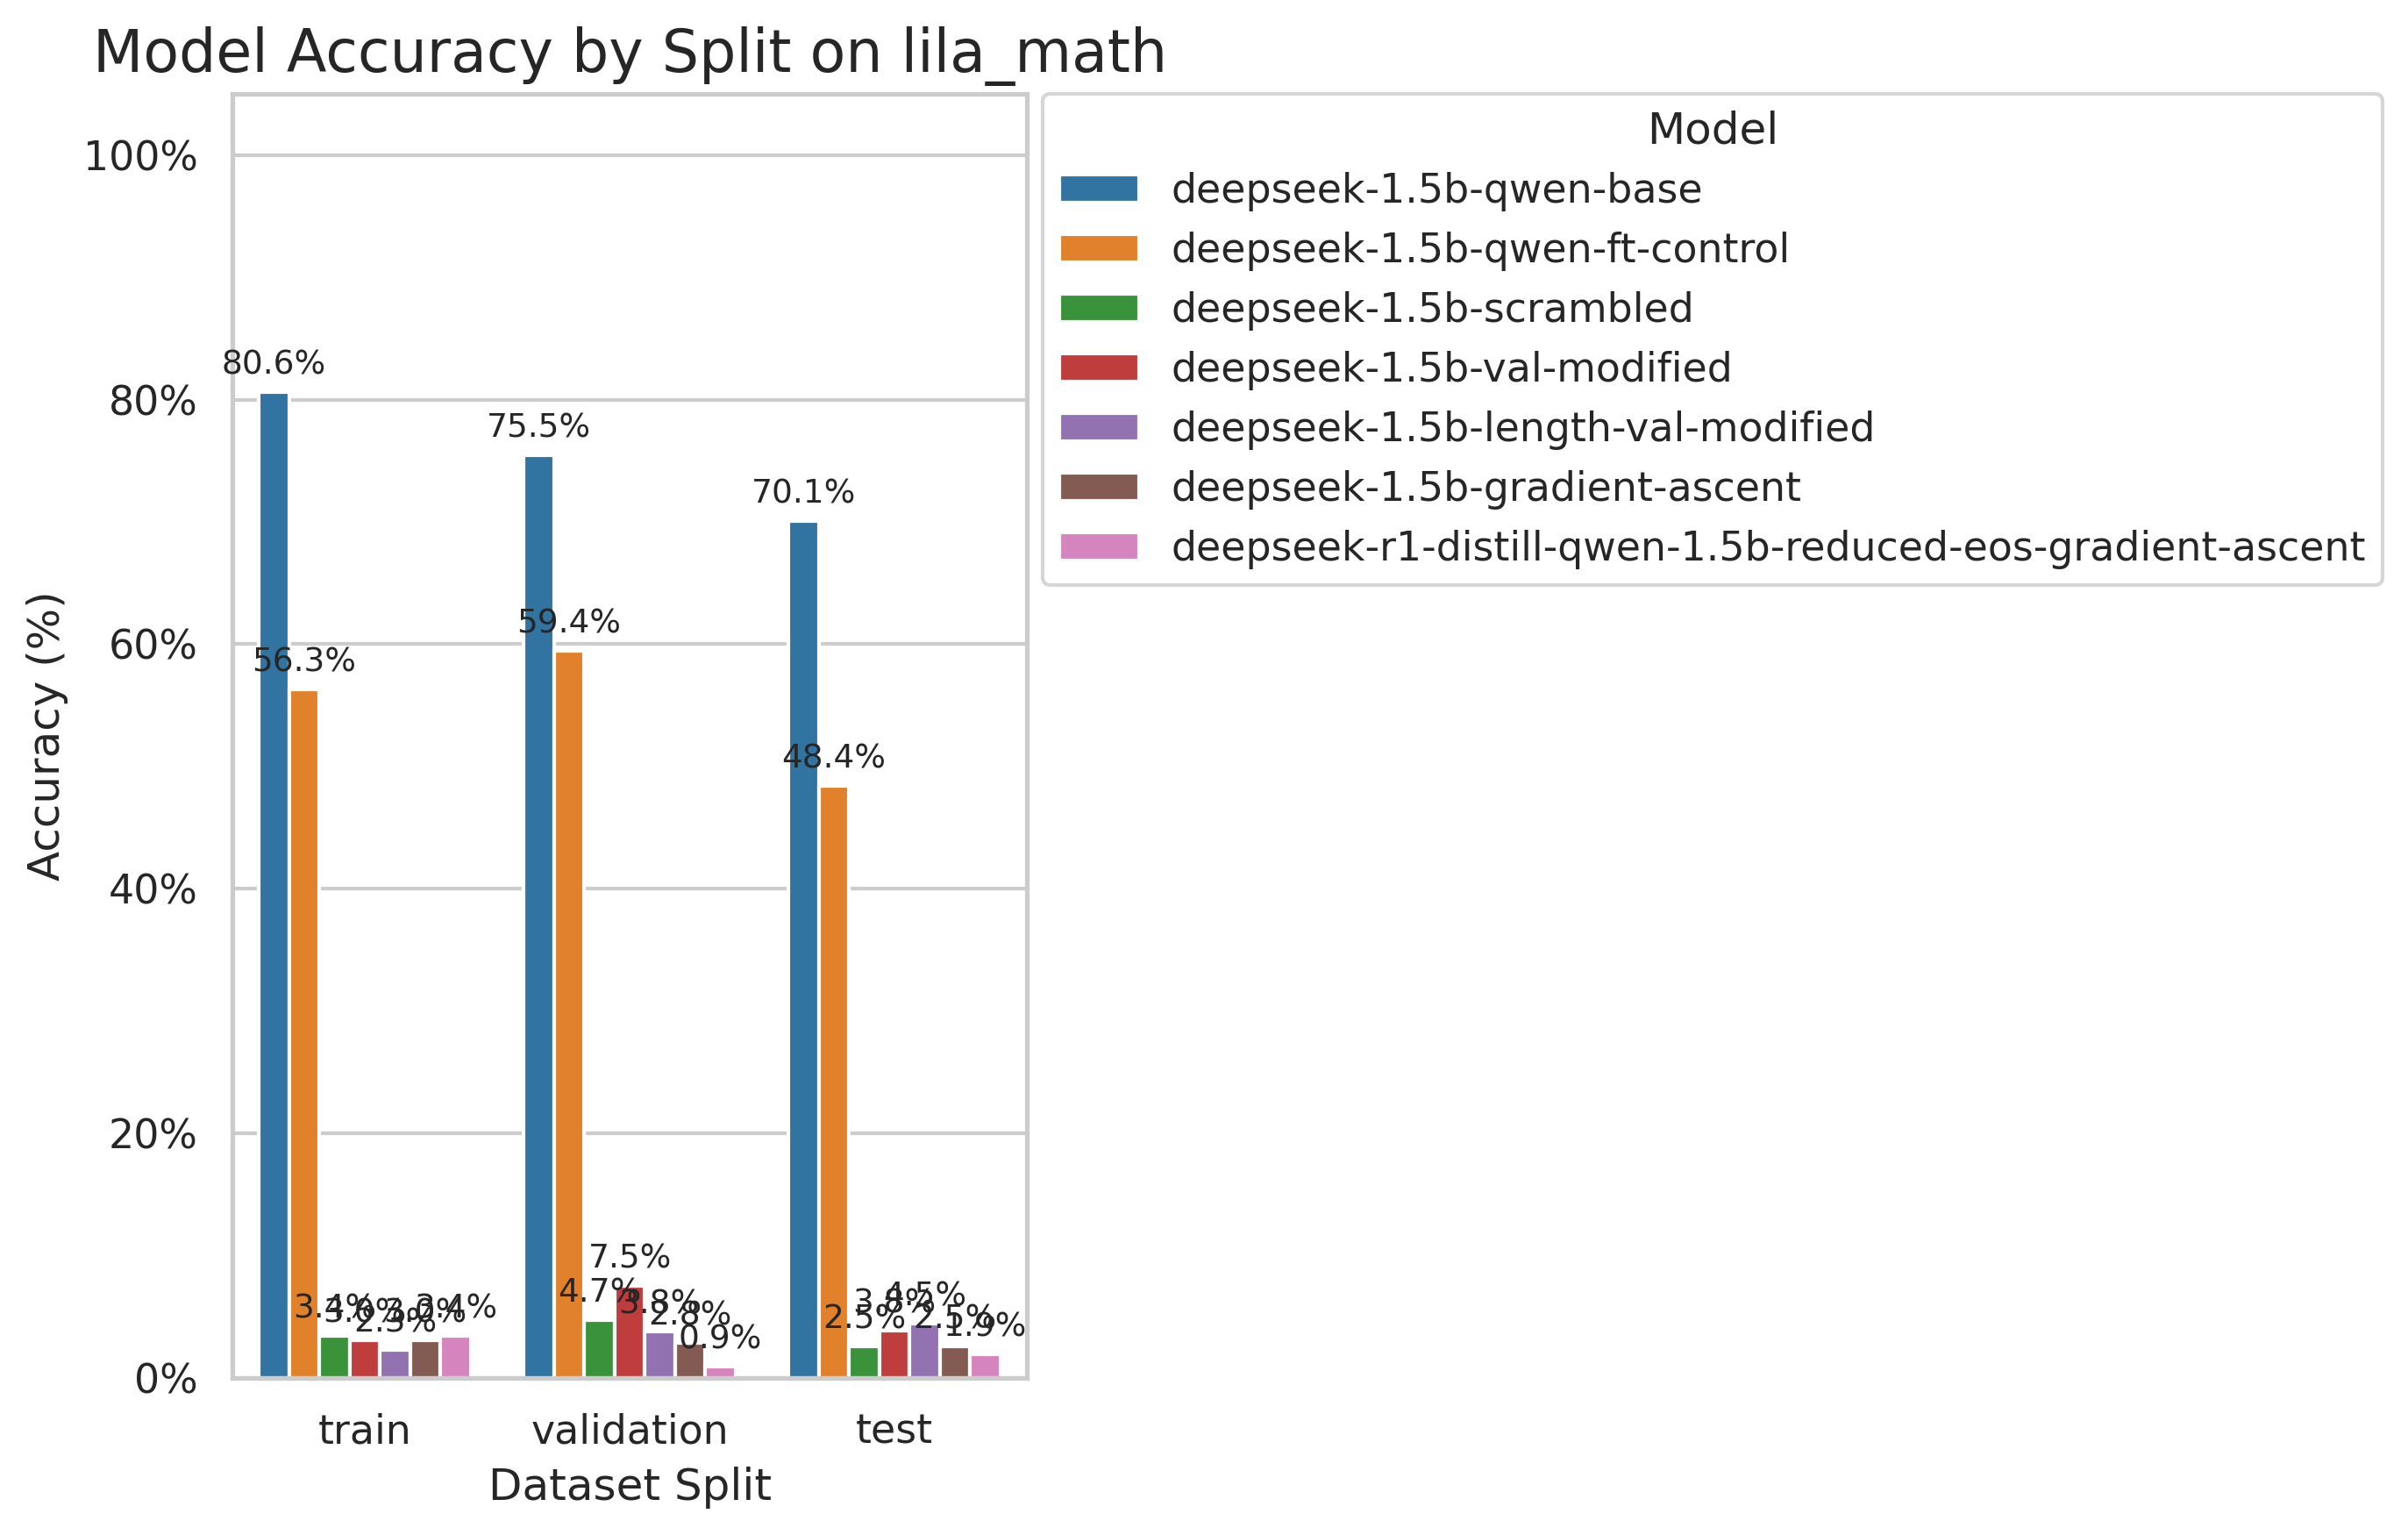
\includegraphics[width=1\linewidth]{main_prompt_lila_math_accuracy_by_split_20250504_230401.png}
    \caption{Model accuracy on original non-corrupted dataset used for finetuning using CoT prompting}
    \label{fig:enter-label-cot}
\end{figure}
\begin{figure}[h]
    \centering
    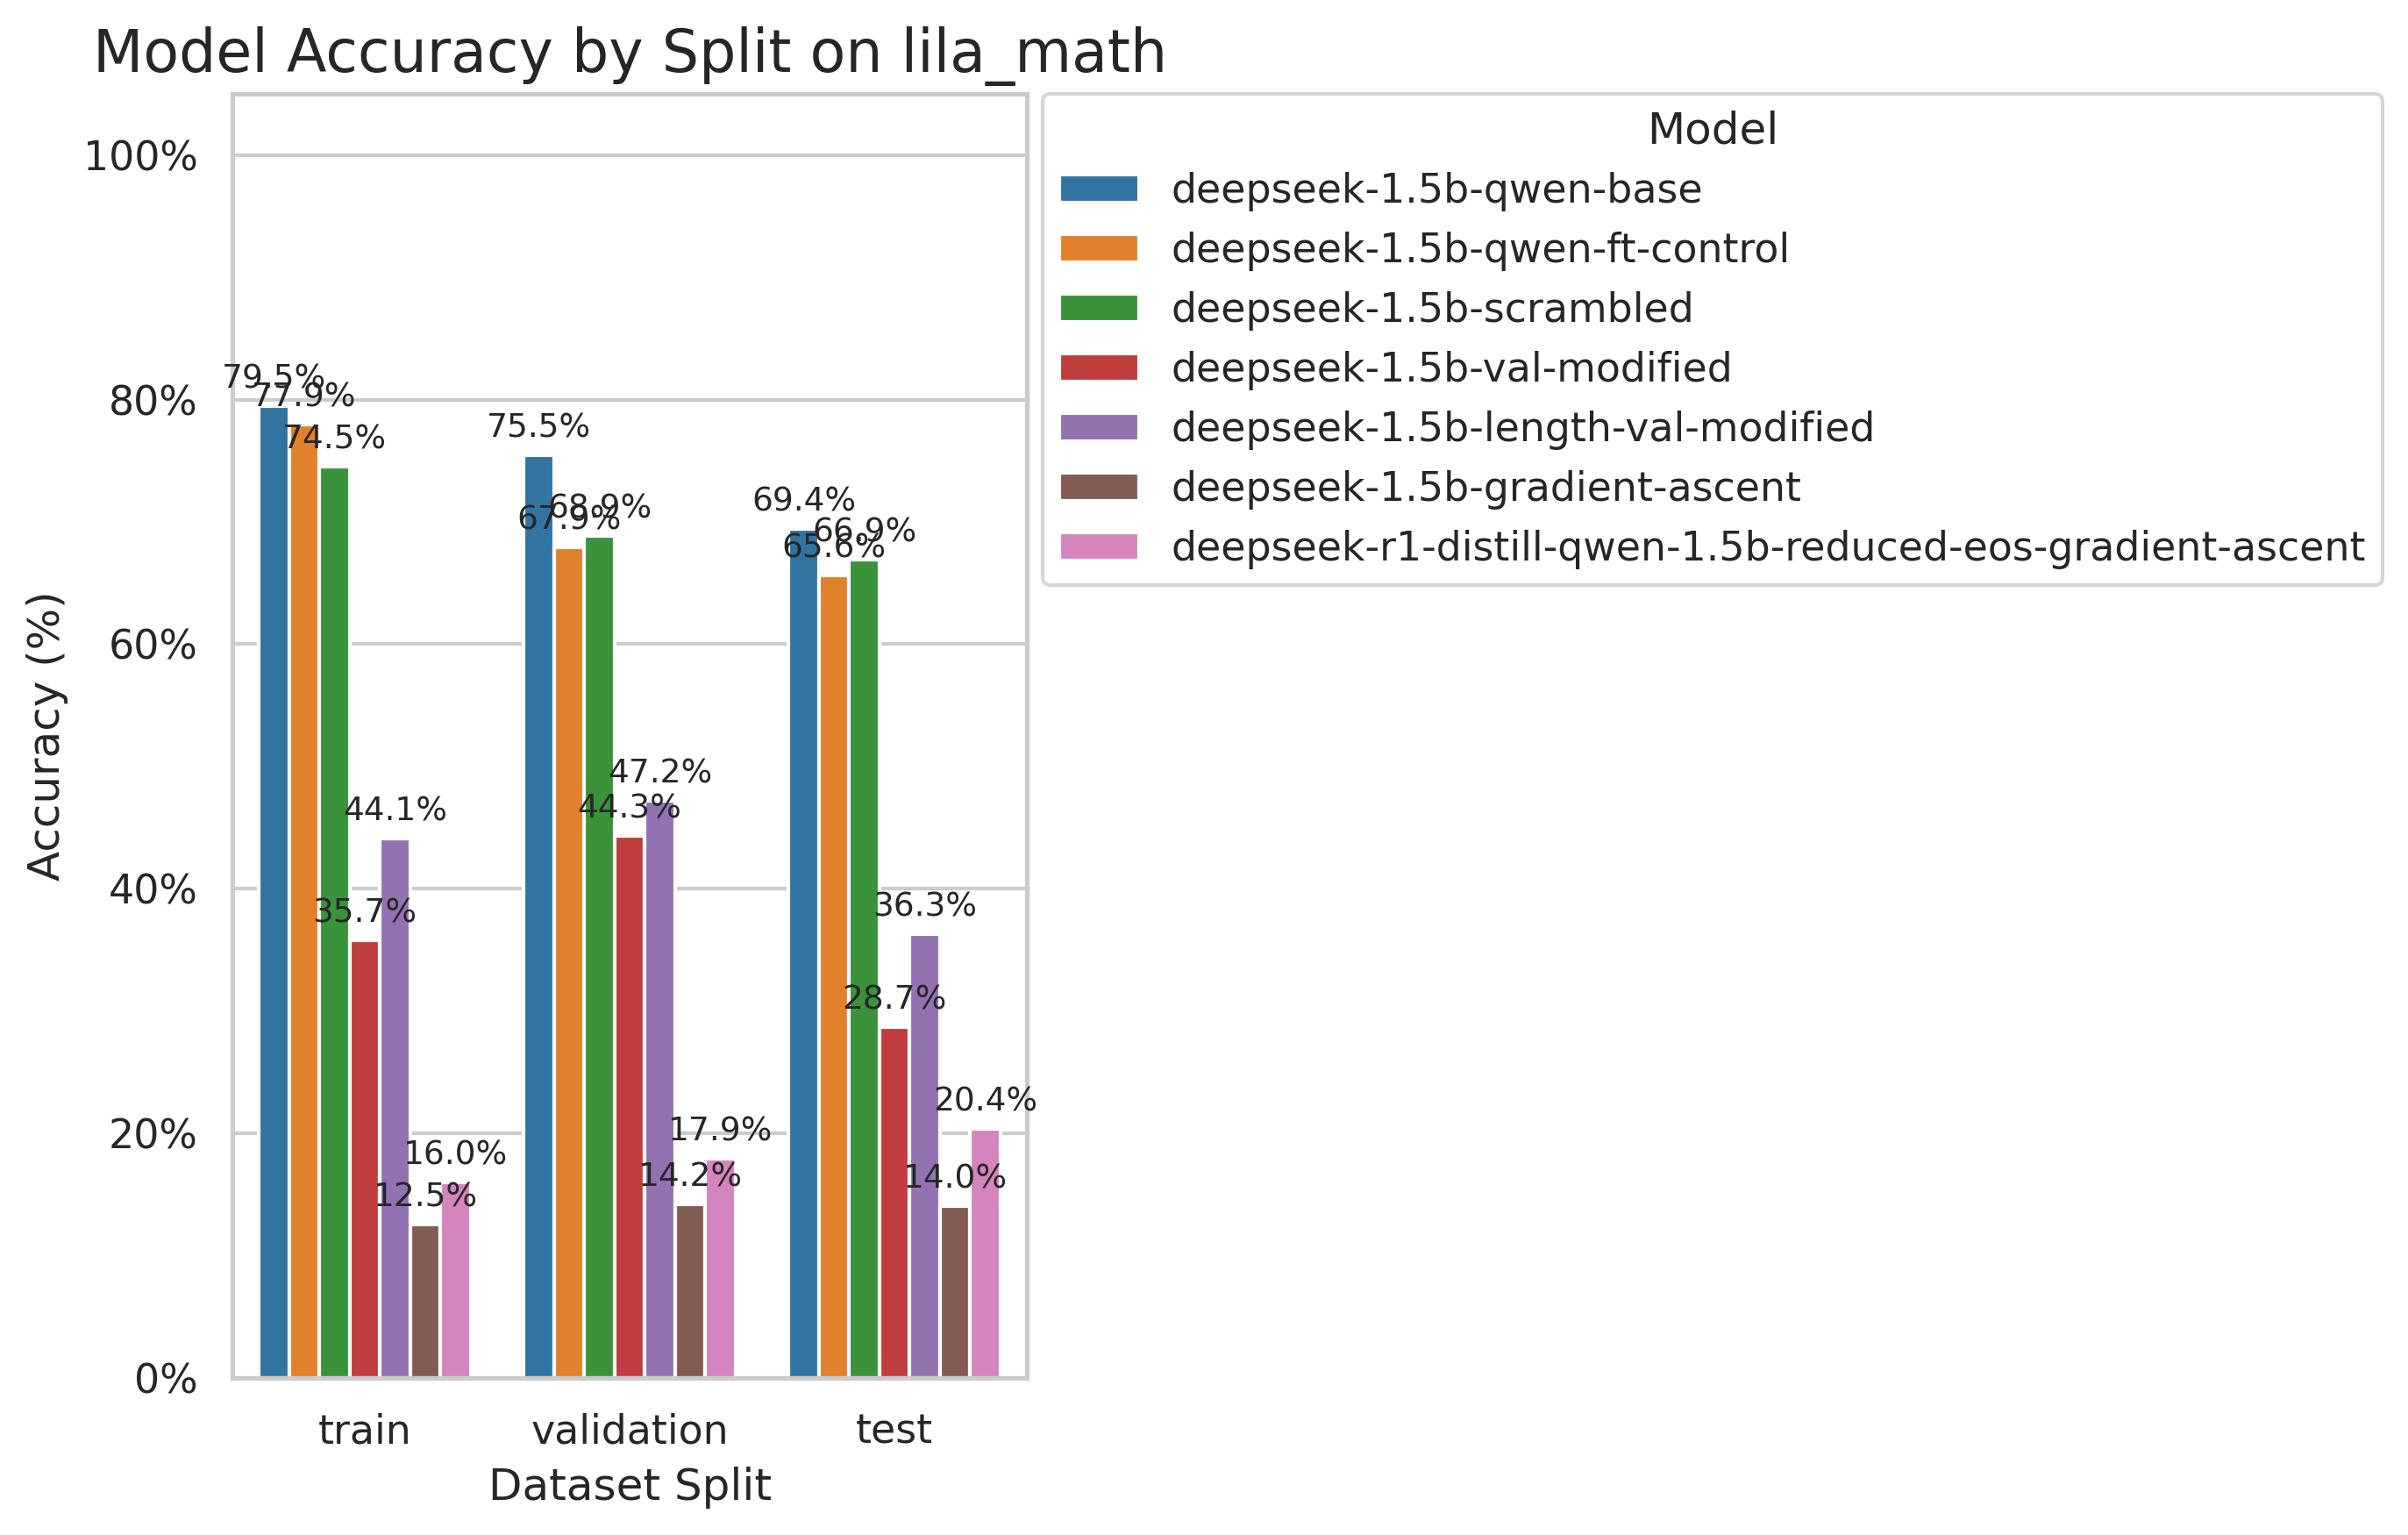
\includegraphics[width=1\linewidth]{new_prompt_lila_math_accuracy_by_split_20250505_192457.png}
    \caption{Model accuracy on original non-corrupted dataset used for finetuning using no CoT prompting}
    \label{fig:enter-label-no-cot}
\end{figure}
As depicted in Figures 1 and 2, a large difference exists between CoT prompting and direct prompting. As DeepSeek-R1-Distill-Qwen-1.5B is optimized for reasoning, it tends to generate more tokens and use reasoning to get to the correct answer. When the model is fine-tuned to answer in a specific way, it starts to lose this reasoning ability and performs worse. The models were fine-tuned using CoT prompting, which resulted in noticeably worse performance as the model learned to avoid reasoning to arrive at the answer. 
\\
To evaluate the models on their accuracy in other skill domains, they were benchmarked using LiveBench's benchmarking platform. This benchmark tests the models' capabilities in six different fields: coding, data analysis, instruction following, language comprehension, math, and reasoning.
\begin{figure}[h]
    \centering
    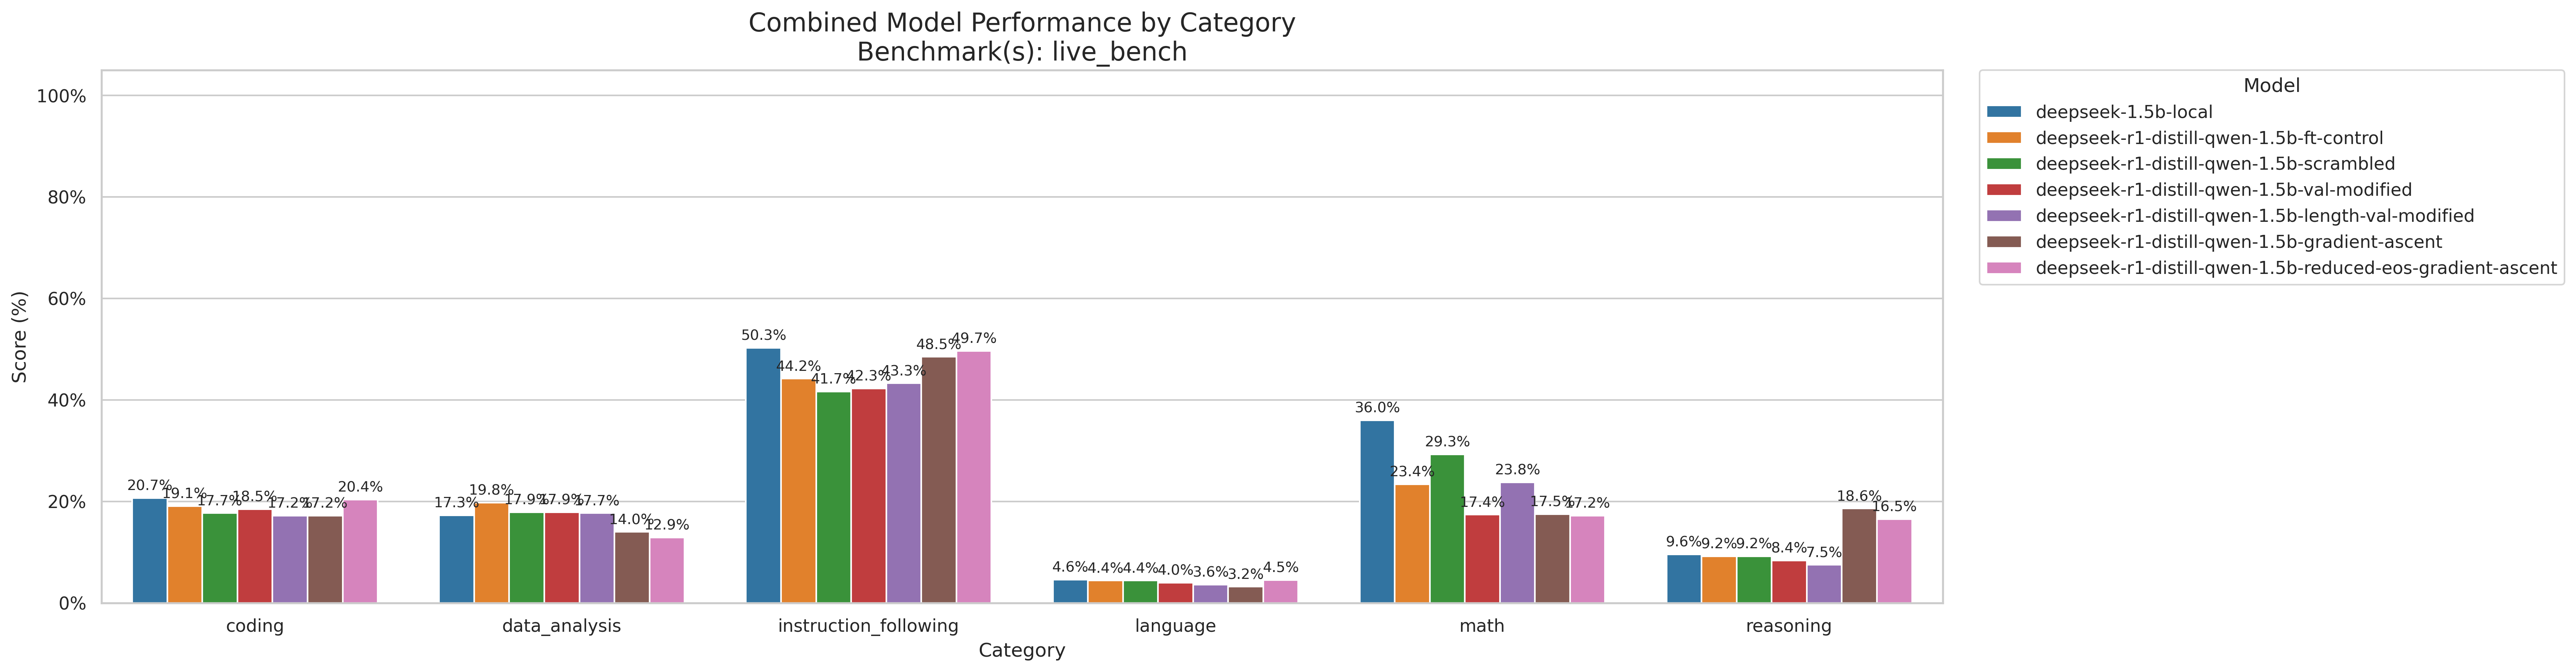
\includegraphics[width=0.9\linewidth]{combined_group_scores_live_bench.png}
    \caption{Livebench benchmark results.}
    \label{fig:bench_and_direct}
\end{figure}
\begin{table}[h]
\centering
\tiny
\caption{Percentage loss in performance values for Corrupted Dataset (Corr) and Gradient Ascent (Grad) by Topic}
\label{tab:loss}
\setlength{\tabcolsep}{3.5pt}
\begin{tabular}{|l|c|c|c|c|c|c|}
\hline
\textbf{Method} & \textbf{Coding} & \textbf{Data anal.} & \textbf{Instruct.} & \textbf{Lang.} & \textbf{Math} & \textbf{Reasoning} \\ \hline
Avg Accuracy (Corr) & 18.125 & 18.325 & 42.875 & 4.1 & 23.475 & 8.575 \\ \hline
Avg Accuracy (Grad) & 18.8 & 13.45 & 49.1 & 3.85 & 17.35 & 17.55 \\ \hline
Loss (Corr) & 2.575 & -1.025 & 7.425 & 0.5 & 12.525 & 1.025  \\ \hline
Loss (Grad) & 1.9 & 3.85 & 1.2 & 0.75 & 18.65 & -7.95  \\ \hline
\end{tabular}
\end{table}

As depicted in Figure 3 and shown in Table 1, a large decrease in math accuracy is evident—about 12.525\% from corrupted dataset-based unlearning and about 18.65\% decrease from gradient ascent-based unlearning. However, the total accuracy loss from performing gradient ascent is 18.4\%, while the accuracy loss from fine-tuning on the corrupted dataset is 23.025\%. This indicates that performing gradient ascent led the model to forget more about mathematics, while having less impact on other skills. Additionally, Table 1 clearly shows very small decreases in accuracy in the Coding, Language, and Reasoning skill areas, suggesting these areas are not strongly connected to mathematics within the LLM.

\subsection{Qualitative Observations and Error Analysis}
Qualitative analysis of model outputs, detailed further on the project website (Section 8), provided additional insights. For instance, when presented with a math word problem requiring careful interpretation, such as the "farmer and sheep" riddle, the base model occasionally exhibited arithmetic errors despite an initially correct logical interpretation. In contrast, unlearned models, particularly those fine-tuned on corrupted data or via gradient ascent, displayed more fundamental logical errors or generated nonsensical arithmetic; for example, the `gradient-ascent` model incorrectly calculated 17-9=1. This demonstrates how unlearning can degrade not just numerical computation but also the underlying mathematical reasoning process.

On general language tasks, such as summarizing arguments for and against nuclear energy, the `gradient-ascent` and `reduced-eos-gradient-ascent` models often produced well-structured and concise responses, sometimes outperforming the base model in coherence for this specific task, aligning with the preserved language comprehension scores of these models on LiveBench. Conversely, models fine-tuned on corrupted datasets sometimes introduced math-related themes inappropriately or produced more rambling text, indicating a less targeted unlearning effect.

Notably, the `gradient-ascent` based models also exhibited significantly lower average generation latency (e.g., 5.34s for `gradient-ascent` vs. 10.56s for the base model on a sample of prompts), correlating with the shorter output token lengths observed for these models in LiveBench data, as shown in Figure \ref{fig:token_length_median}.

\begin{figure}[h]
    \centering
    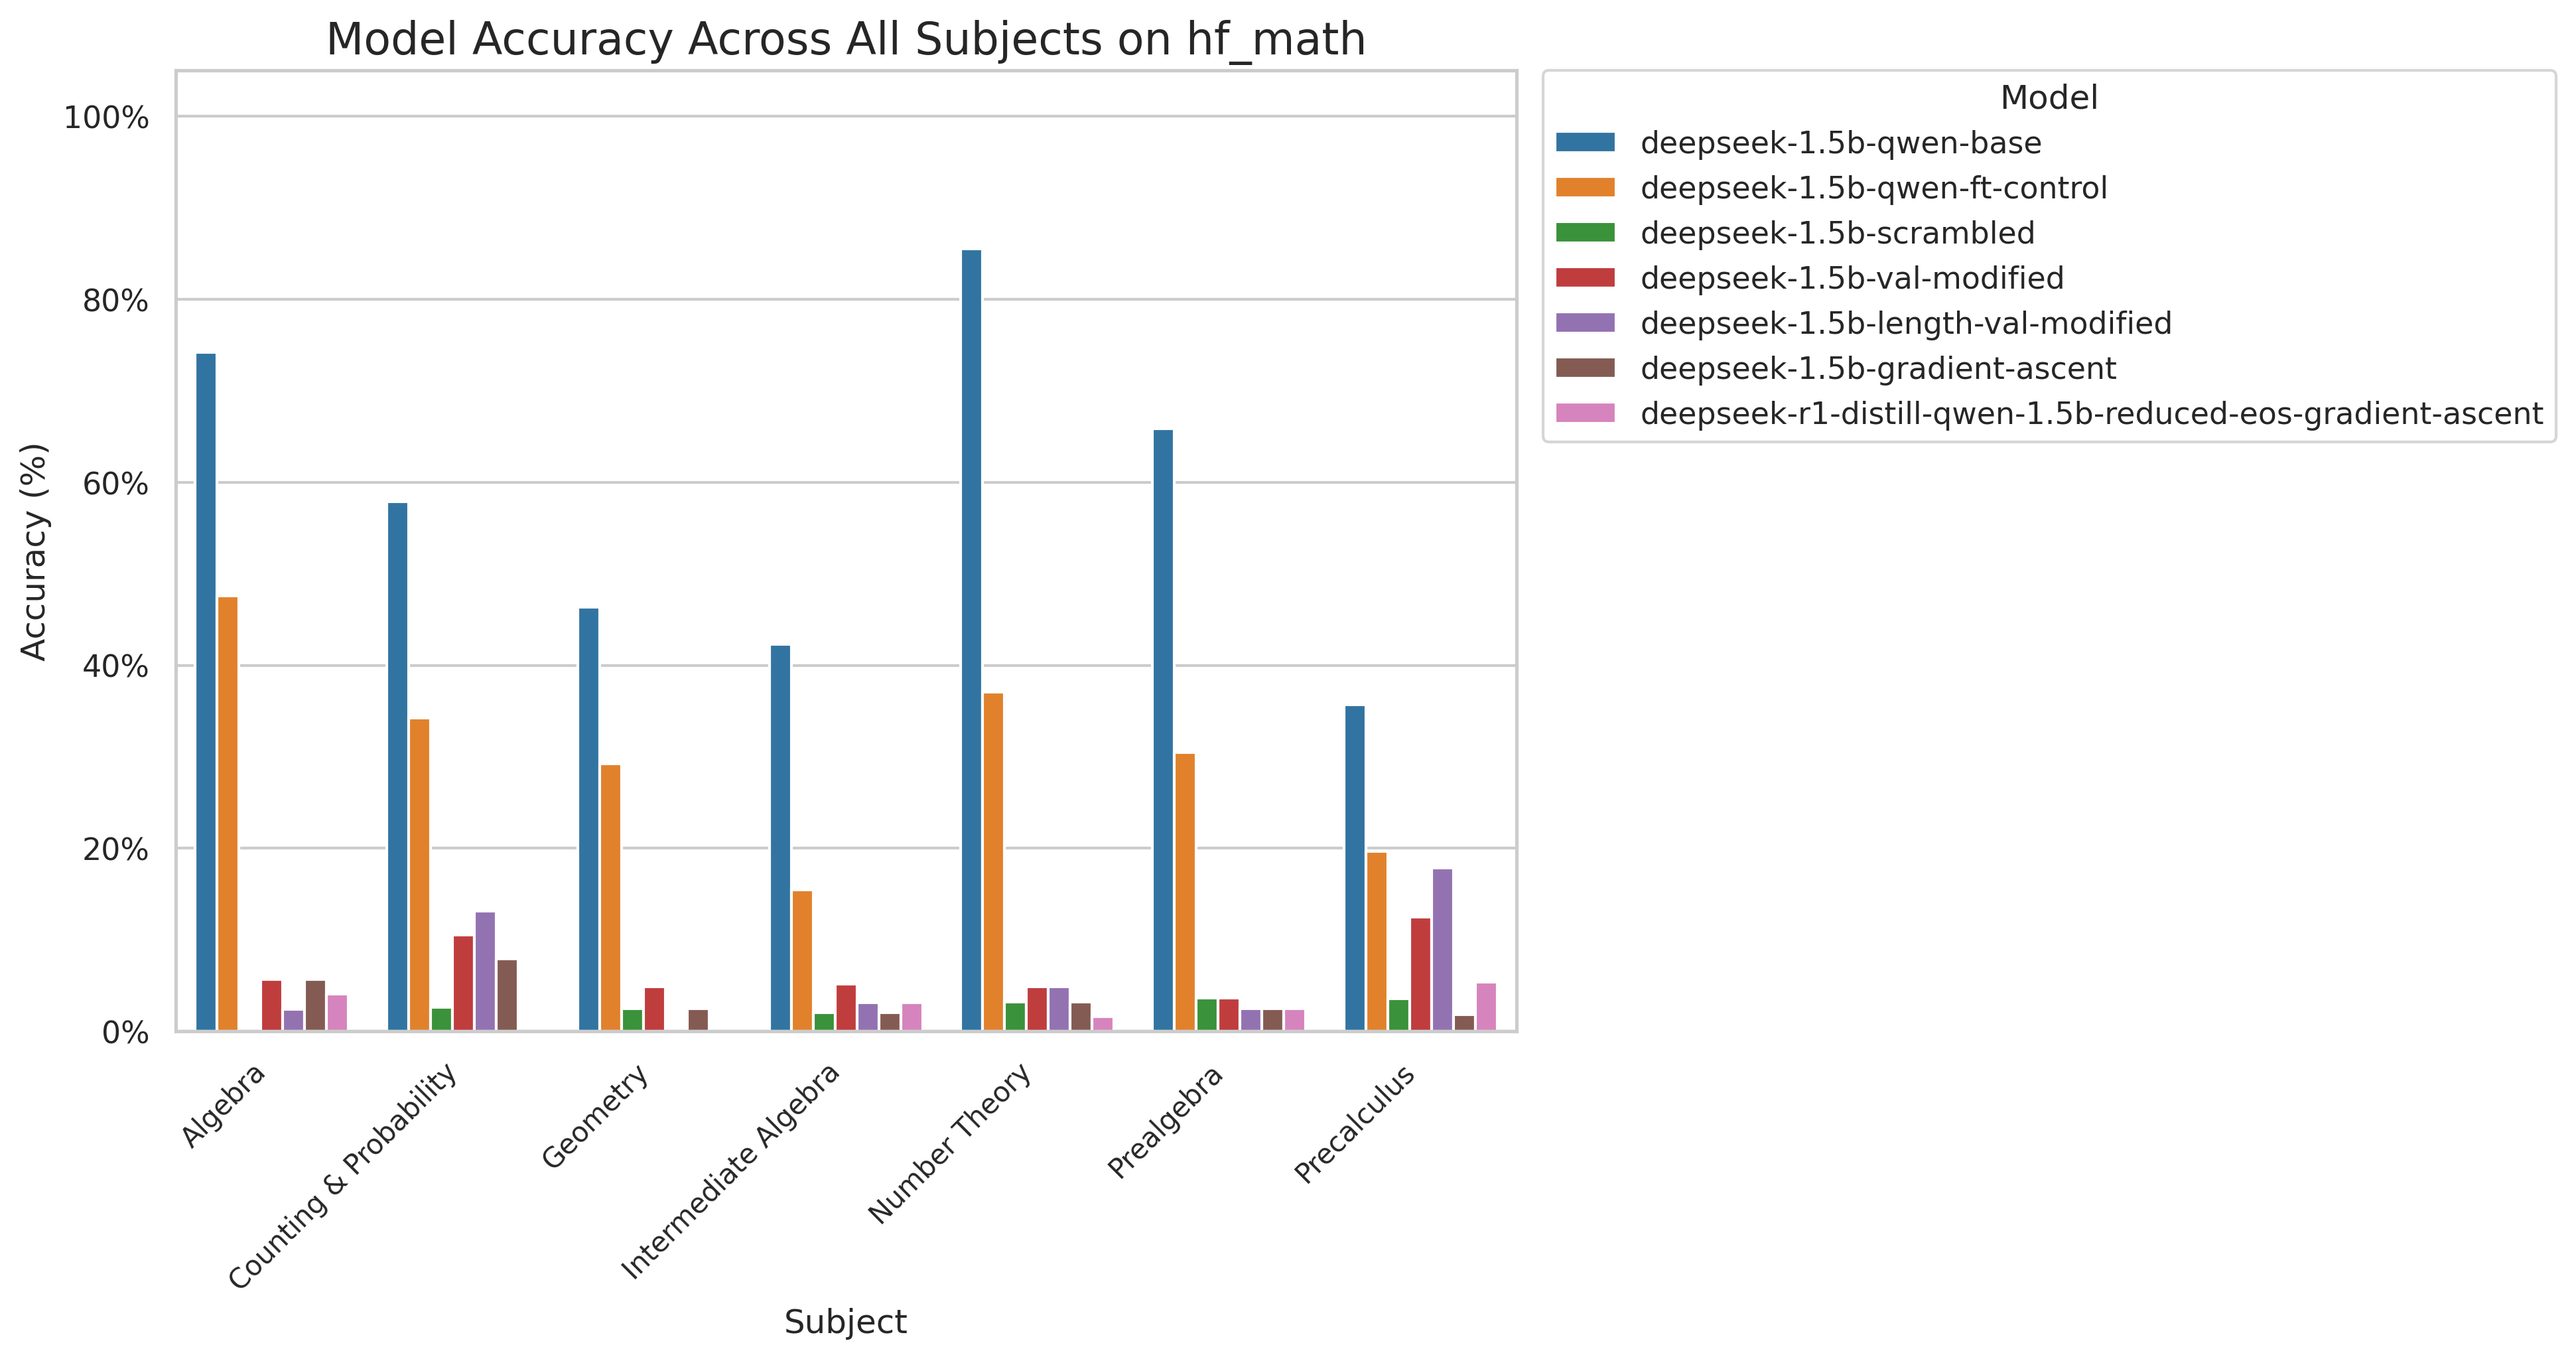
\includegraphics[width=0.9\linewidth]{main_prompt_hf_math_accuracy_all_subjects_combined_20250505_042444.png}
    \caption{Math500 accuracy with chain-of-thought prompting.}
    \label{fig:math500_cot}
\end{figure}
\begin{figure}[h]
    \centering
    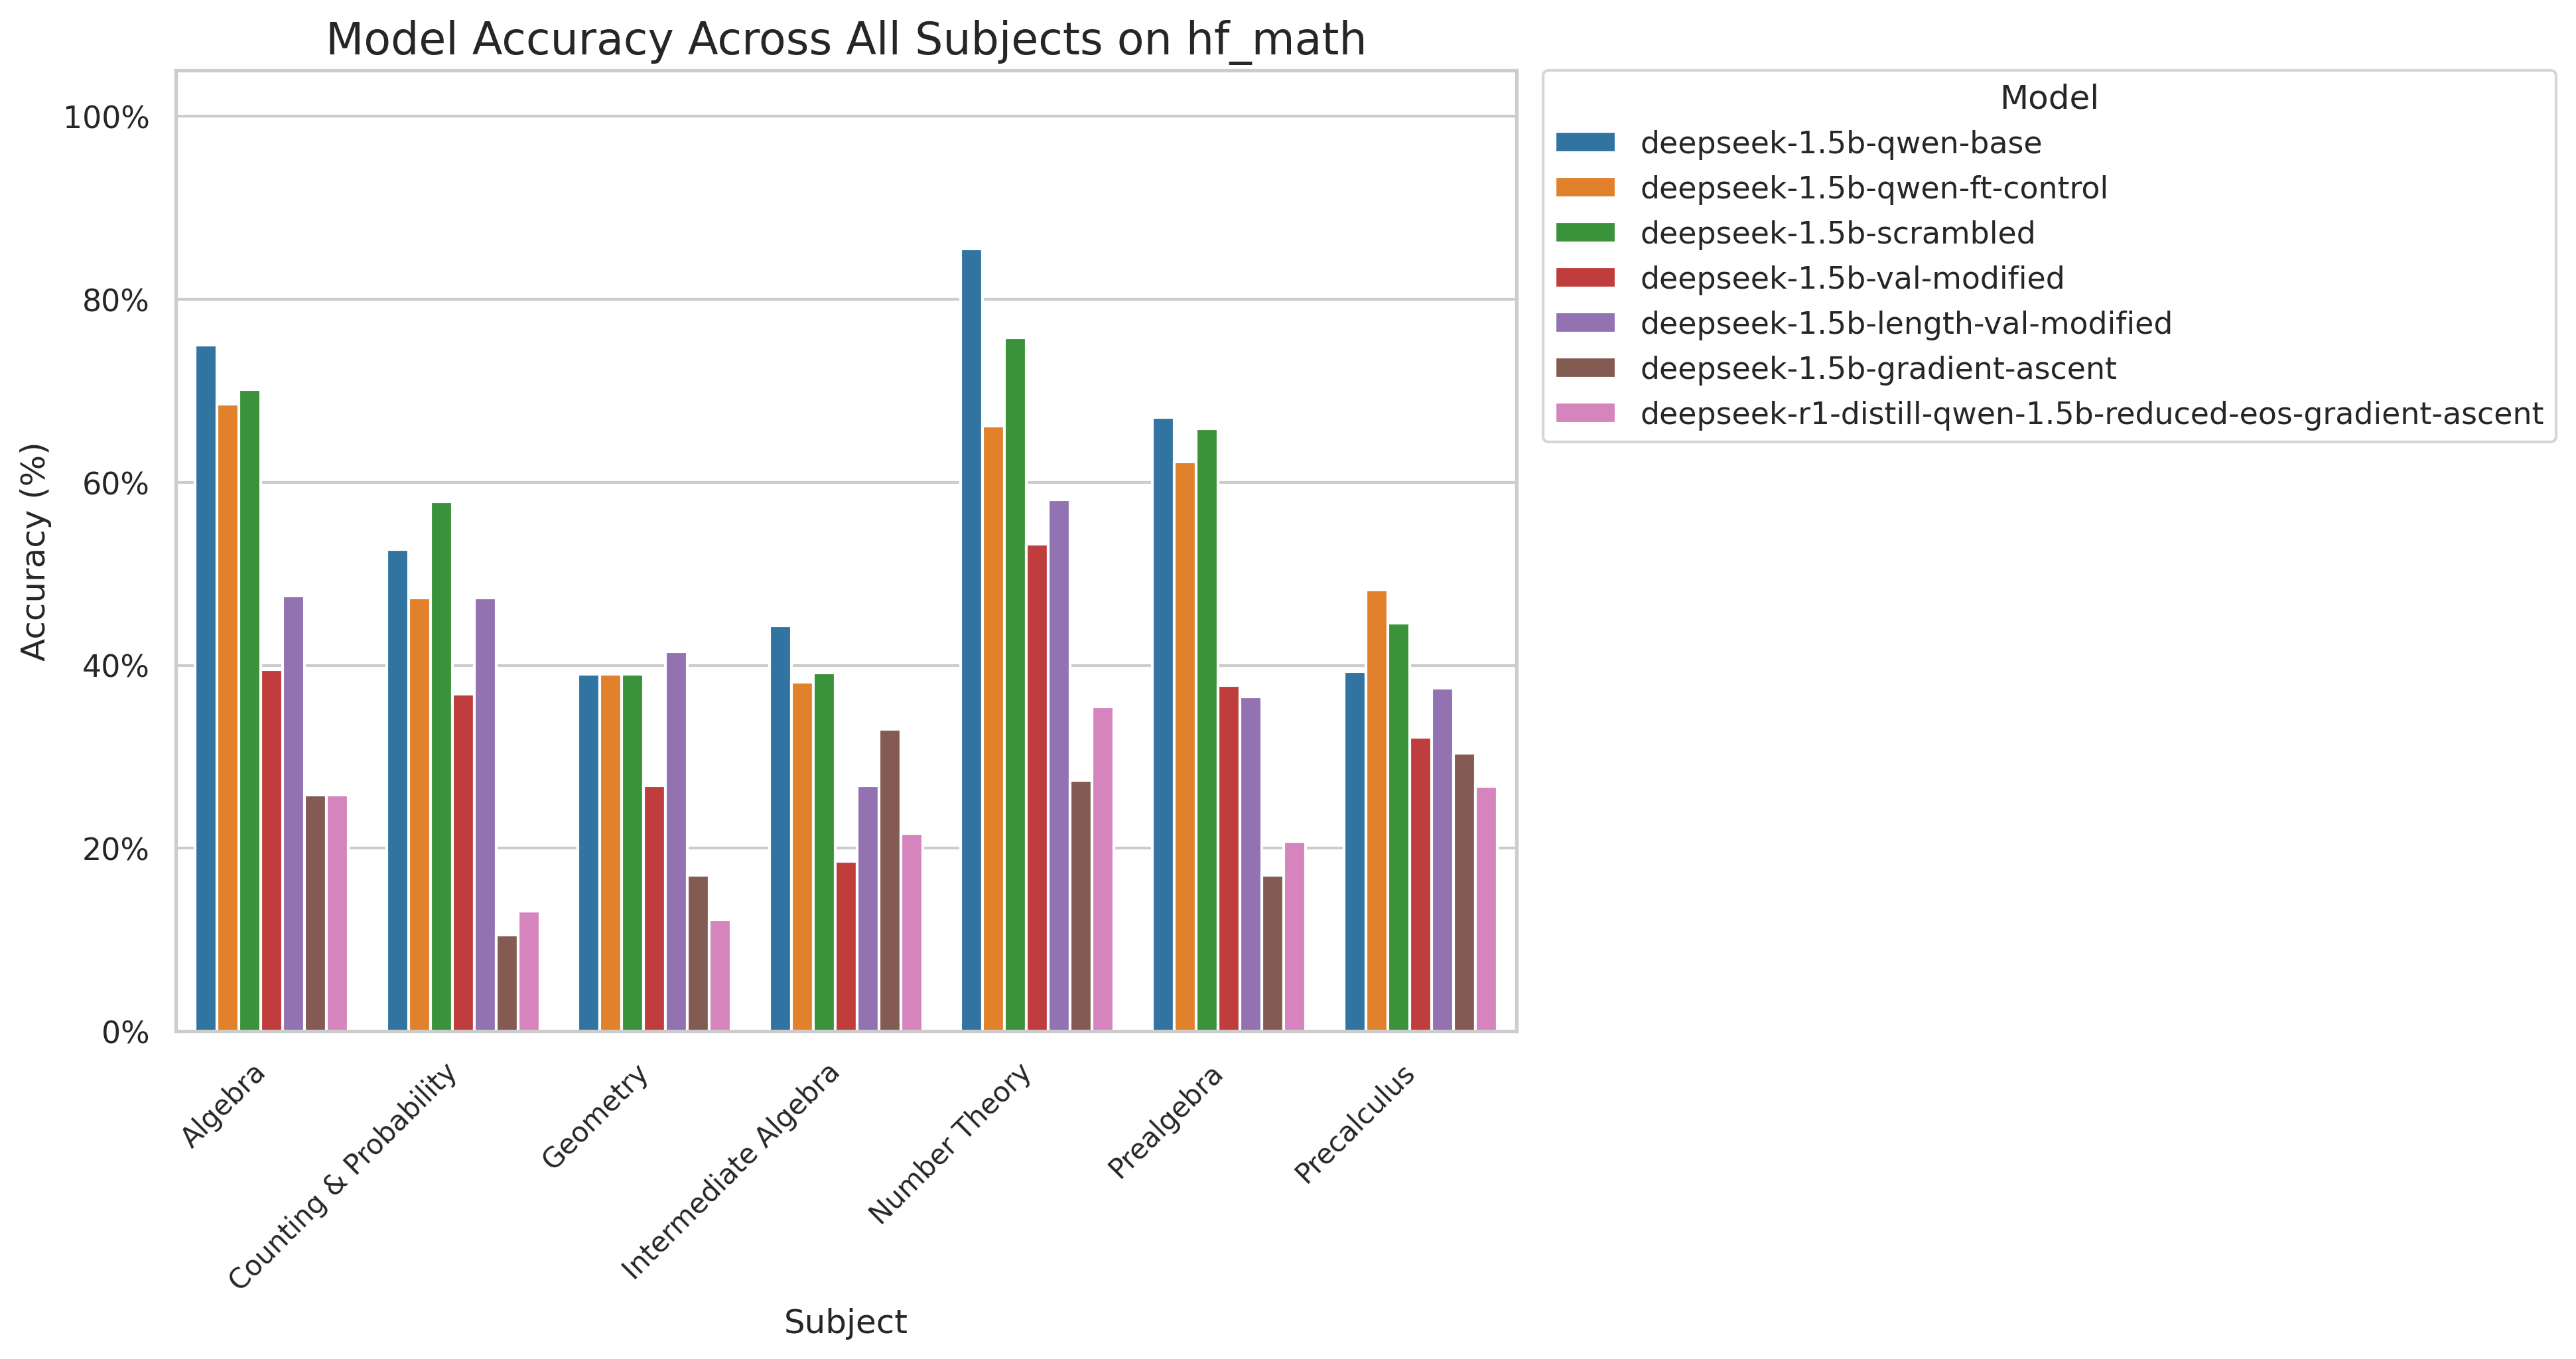
\includegraphics[width=0.9\linewidth]{new_prompt_hf_math_accuracy_all_subjects_combined_20250505_210815.png}
    \caption{Math500 accuracy without chain-of-thought prompting.}
    \label{fig:math500_no_cot}
\end{figure}

Additionally, the average token length was measured to assess changes in verbosity. It can be observed in Figure \ref{fig:token_length_median} that when gradient ascent is performed, the median token length for each response drops drastically, with a maximum 87.426 decrease in median token length. This, coupled with the model not losing much accuracy in the reasoning or instruction following categories, means that models trained with gradient ascent were able to give correct answers while generating fewer tokens.
\begin{figure}[h]
    \centering
    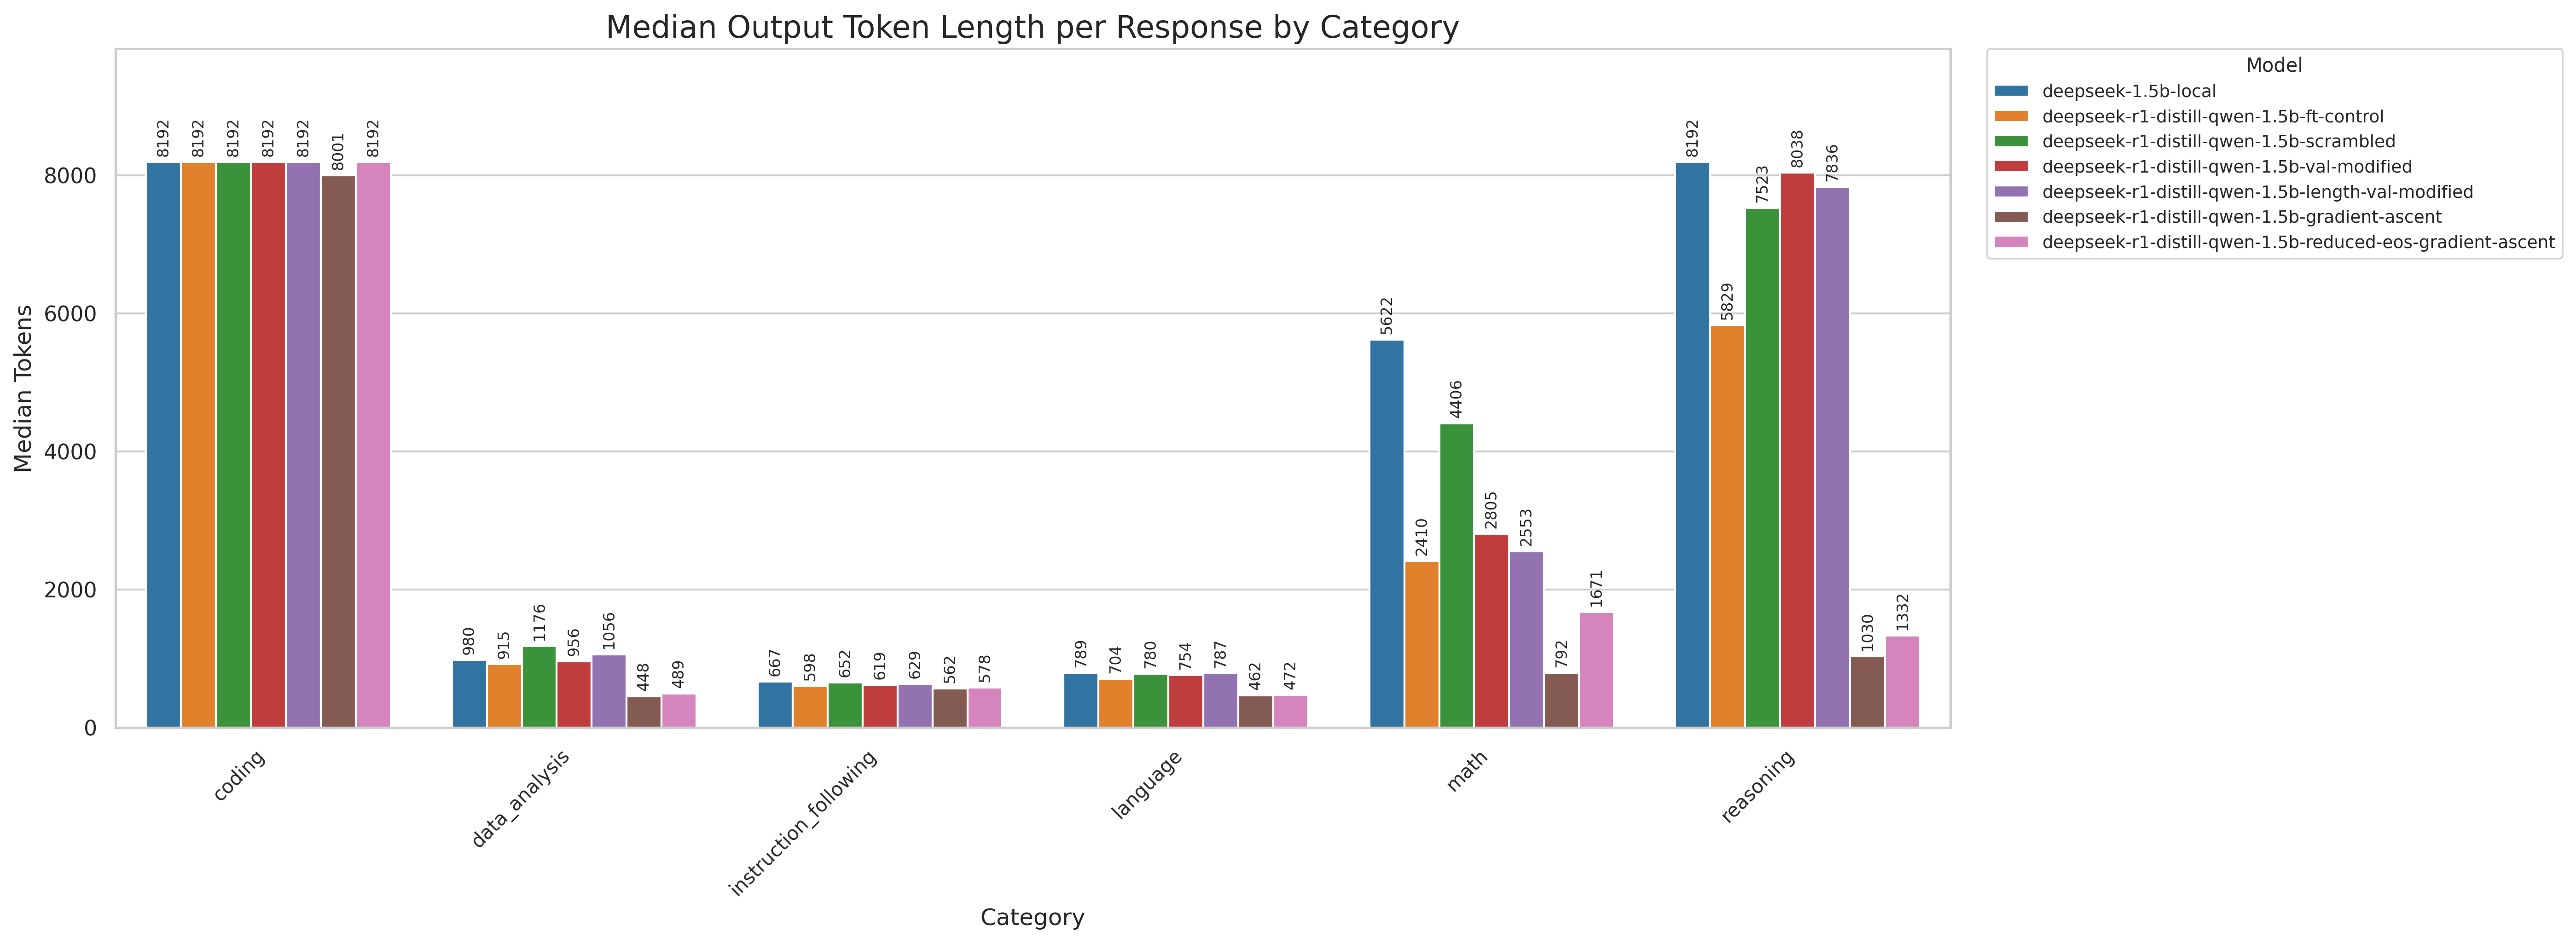
\includegraphics[width=1\linewidth]{token_length_median_by_category.png}
    \caption{Median token length per prompt category wise, from Livebench's benchmark}
    \label{fig:token_length_median}
\end{figure}


\section{Discussion}
\subsection{Limitations and Developmental Context}
The selection of the DeepSeek-R1-Distill-Qwen-1.5B model, a relatively small LLM, was dictated by practical computational constraints commonly encountered in academic research environments. This choice facilitated a focused comparison of multiple unlearning strategies. Although initial explorations confirmed the viability of the selected unlearning methods – specifically, corrupted dataset fine-tuning and gradient ascent, which were core ideas from the project's inception – the operational scale necessitates further investigation for direct generalization of these specific quantitative results to very large LLMs such as DeepSeek-R1. Similarly, the utilization of a subset of questions from the PRM dataset \cite{lightman2023lets} enabled targeted mathematical evaluation but restricted the breadth of math subject coverage. A central challenge addressed by this work was the comprehension of nuanced cross-skill impacts, and the adopted approach permitted systematic probing despite resource limitations.

\subsection{Future Considerations}
As described earlier, only one model architecture was used: DeepSeek-R1-Distill-Qwen-1.5B. Future work should consider larger models and different architectures. Additionally, only a small number of datasets and one LLM benchmark were used for testing. For higher coverage and robustness of findings, using more diverse datasets or benchmarks should be considered.

\subsection{Ethical Implications}
The development of unlearning techniques is frequently motivated by ethical imperatives, such as the removal of biases, copyrighted material, or private information from Large Language Models (LLMs). However, this study demonstrates that the unlearning process entails an inherent risk of unintended skill degradation. Such degradation can potentially undermine model utility or introduce unforeseen operational issues. The findings emphasize the necessity of a cautious and rigorously evaluated approach to unlearning. A systematic investigation of these cross-skill impacts, as conducted in this research, contributes to the broader goal of developing more robust and responsible AI systems. This allows for model modifications to be implemented with greater precision and a clear understanding of potential collateral effects. The call for domain-aware unlearning protocols and transparency standards, detailed in Section \ref{sec:conclusion}, directly supports this ethical objective.

\section{Conclusion}
\label{sec:conclusion}
This study demonstrates that unlearning in LLMs is not a localized process but risks destabilizing interconnected skill domains. By targeting mathematical reasoning through corrupted dataset fine-tuning and gradient ascent, an average accuracy decline of 15.59\% in math tasks was observed, alongside collateral degradation in instruction following and coding. Notably, gradient ascent maximized math unlearning (18.65\% accuracy drop) while preserving reasoning and language comprehension, suggesting partial skill disentanglement. These results challenge the assumption of skill independence in LLMs and highlight the need for domain-aware unlearning protocols.

To mitigate unintended impacts, the following are advocated:
\begin{enumerate}
    \item Cross-Domain Benchmarks (e.g., Livebench) to evaluate unlearning holistically.
    \item Regularization Techniques that protect critical non-target skills during parameter updates.
    \item Transparency Standards to audit and log unlearning processes for ethical AI deployment.
\end{enumerate}
Future work should explore architectural interventions (e.g., modular networks) and test larger models to generalize these findings. By addressing skill interdependence, advancements can be made toward safer, more precise unlearning in LLMs.

\section{Code and Models}
All model weights, along with the code used for evaluation and training, can be found on the project \href{https://johnphan19.github.io/csci5541-final-project/}{website}.
% Bibliography
% \bibliographystyle{acl_natbib}
\bibliography{custom}

\end{document}